
\begin{figure}[H]
  \centering
  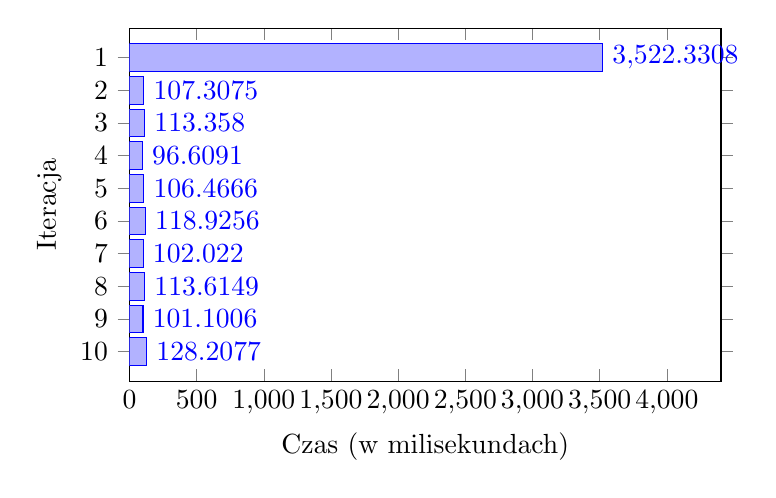
\begin{tikzpicture}
  
    \begin{axis} [
      xbar = .05cm,
      nodes near coords,
      nodes near coords style={
        /pgf/number format/precision=4,
      },
      xmin = 0,
      ytick = data,
      enlarge x limits = {value = .25, upper},
      symbolic y coords = {10,9,8,7,6,5,4,3,2,1},
      xlabel=Czas (w milisekundach),
      ylabel=Iteracja,
      width=0.75\textwidth,
      height=0.5\textwidth
    ]
    
      \addplot coordinates {(3522.330799996853,1) (107.30750000476837,2) (113.35799998044968,3) (96.609099984169,4) (106.4666000008583,5) (118.92559999227524,6) (102.02200001478195,7) (113.61489999294281,8) (101.10060000419617,9) (128.20770001411438,10)};
      
    \end{axis}
  
  \end{tikzpicture}
  \caption{Wynik testów przykładu 6 [\ref{lst:wydajnosc-przyklad-p-6}]}
  \label{fig:wynik-przyklad-5}
\end{figure}
